%%%%%%%%%%%%%%%%%%%%%%%%%%%%%%%%%%%%%%%%%%%%%%
%% Compile: XeLaTeX BibTeX XeLaTeX XeLaTeX
%% Loesung-Handout: Antonio Machicao y Priemer
%% Course: GK Linguistik
%%%%%%%%%%%%%%%%%%%%%%%%%%%%%%%%%%%%%%%%%%%%%%

%\documentclass[a4paper,10pt, bibtotoc]{beamer}
\documentclass[10pt,handout]{beamer}

%%%%%%%%%%%%%%%%%%%%%%%%
%%     PACKAGES      
%%%%%%%%%%%%%%%%%%%%%%%%

%%%%%%%%%%%%%%%%%%%%%%%%
%%     PACKAGES       %%
%%%%%%%%%%%%%%%%%%%%%%%%



%\usepackage[utf8]{inputenc}
%\usepackage[vietnamese, english,ngerman]{babel}   % seems incompatible with german.sty
%\usepackage[T3,T1]{fontenc} breaks xelatex
\usepackage{lmodern}

\usepackage{amsmath}
\usepackage{amsfonts}
\usepackage{amssymb}
%% MnSymbol: Mathematische Klammern und Symbole (Inkompatibel mit ams-Packages!)
%% Bedeutungs- und Graphemklammern: $\lsem$ Tisch $\rsem$ $\langle TEXT \rangle$ $\llangle$ TEXT $\rrangle$ 
\usepackage{MnSymbol}
%% ulem: Strike out
\usepackage[normalem]{ulem}  

%% Special Spaces (s. Commands)
\usepackage{xspace}				
\usepackage{setspace}
%	\onehalfspacing

%% mdwlist: Special lists
\usepackage{mdwlist}	

\usepackage[noenc,safe]{tipa}

% maybe define \textipa to use \originalTeX to avoid problems with `"'.
%
%	\ex \textipa{\originalTeX [pa.pa."g\t{aI}]}

%

\usepackage{etex}		%For Forest bug

%
%\usepackage{jambox}
%


%\usepackage{forest-v105}
%\usepackage{modified-langsci-forest-setup}

\usepackage{xeCJK}
\setCJKmainfont{SimSun}


%\usepackage{natbib}
%\setcitestyle{notesep={:~}}




% for toggles
\usepackage{etex}



% Fraktur!
\usepackage{yfonts}

\usepackage{url}

% für UDOP
\usepackage{adjustbox}


%% huberlin: Style sheet
%\usepackage{huberlin}
\usepackage{hu-beamer-includes-pdflatex}
\huberlinlogon{0.86cm}


%% Last Packages
%\usepackage{hyperref}	%URLs
%\usepackage{gb4e}		%Linguistic examples

% sorry this was incompatible with gb4e and had to go.
%\usepackage{linguex-cgloss}	%Linguistic examples (patched version that works with jambox

\usepackage{multirow}  %Mehrere Zeilen in einer Tabelle
%\usepackage{array}
\usepackage{marginnote}	%Notizen




%%%%%%%%%%%%%%%%%%%%%%%%%%%%%%%%%%%%%%%%%%%%%%%%%%%%
%%%          Commands                            %%%
%%%%%%%%%%%%%%%%%%%%%%%%%%%%%%%%%%%%%%%%%%%%%%%%%%%%

%%%%%%%%%%%%%%%%%%%%%%%%%%%%%%%%
% German quotation marks:
\newcommand{\gqq}[1]{\glqq{}#1\grqq{}}		%double
\newcommand{\gq}[1]{\glq{}#1\grq{}}			%simple


%%%%%%%%%%%%%%%%%%%%%%%%%%%%%%%%
% Abbreviations in German
% package needed: xspace
% Short space in German abbreviations: \,	
\newcommand{\idR}{\mbox{i.\,d.\,R.}\xspace}
\newcommand{\su}{\mbox{s.\,u.}\xspace}
%\newcommand{\ua}{\mbox{u.\,a.}\xspace}       % in abbrev
%\newcommand{\zB}{\mbox{z.\,B.}\xspace}       % in abbrev
%\newcommand{\s}{s.~}
%not possibel: \dh --> d.\,h.


%%%%%%%%%%%%%%%%%%%%%%%%%%%%%%%%
%Abbreviations in English
\newcommand{\ao}{a.o.\ }	% among others
\newcommand{\cf}[1]{(cf.~#1)}	% confer = compare
\renewcommand{\ia}{i.a.}	% inter alia = among others
\newcommand{\ie}{i.e.~}	% id est = that is
\newcommand{\fe}{e.g.~}	% exempli gratia = for example
%not possible: \eg --> e.g.~
\newcommand{\vs}{vs.\ }	% versus
\newcommand{\wrt}{w.r.t.\ }	% with respect to


%%%%%%%%%%%%%%%%%%%%%%%%%%%%%%%%
% Dash:
\newcommand{\gs}[1]{--\,#1\,--}


%%%%%%%%%%%%%%%%%%%%%%%%%%%%%%%%
% Rightarrow with and without space
\def\ra{\ensuremath\rightarrow}			%without space
\def\ras{\ensuremath\rightarrow\ }		%with space


%%%%%%%%%%%%%%%%%%%%%%%%%%%%%%%%
%% X-bar notation

%% Notation with primes (not emphasized): \xbar{X}
\newcommand{\MyPxbar}[1]{#1$^{\prime}$}
\newcommand{\xxbar}[1]{#1$^{\prime\prime}$}
\newcommand{\xxxbar}[1]{#1$^{\prime\prime\prime}$}

%% Notation with primes (emphasized): \exbar{X}
\newcommand{\exbar}[1]{\emph{#1}$^{\prime}$}
\newcommand{\exxbar}[1]{\emph{#1}$^{\prime\prime}$}
\newcommand{\exxxbar}[1]{\emph{#1}$^{\prime\prime\prime}$}

% Notation with zero and max (not emphasized): \xbar{X}
\newcommand{\zerobar}[1]{#1$^{0}$}
\newcommand{\maxbar}[1]{#1$^{\textsc{max}}$}

% Notation with zero and max (emphasized): \xbar{X}
\newcommand{\ezerobar}[1]{\emph{#1}$^{0}$}
\newcommand{\emaxbar}[1]{\emph{#1}$^{\textsc{max}}$}

%% Notation with bars (already implemented in gb4e):
% \obar{X}, \ibar{X}, \iibar{X}, \mbar{X} %Problems with \mbar!
%
%% Without gb4e:
\newcommand{\overbar}[1]{\mkern 1.5mu\overline{\mkern-1.5mu#1\mkern-1.5mu}\mkern 1.5mu}
%
%% OR:
\newcommand{\MyPibar}[1]{$\overline{\textrm{#1}}$}
\newcommand{\MyPiibar}[1]{$\overline{\overline{\textrm{#1}}}$}
%% (emphasized):
\newcommand{\eibar}[1]{$\overline{#1}$}
\newcommand{\eiibar}[1]{\overline{$\overline{#1}}$}

%%%%%%%%%%%%%%%%%%%%%%%%%%%%%%%%
%% Subscript & Superscript: no italics
\newcommand{\MyPdown}[1]{$_{\textrm{#1}}$}
\newcommand{\MyPup}[1]{$^{\textrm{#1}}$}


%%%%%%%%%%%%%%%%%%%%%%%%%%%%%%%%
% Objekt language marking:
%\newcommand{\obj}[1]{\glqq{}#1\grqq{}}	%German double quotes
%\newcommand{\obj}[1]{``#1''}			%English double quotes
\newcommand{\MyPobj}[1]{\emph{#1}}		%Emphasising


%%%%%%%%%%%%%%%%%%%%%%%%%%%%%%%%
%% Semantic types (<e,t>), features, variables and graphemes in angled brackets 

%%% types and variables, in math mode: angled brackets + italics + no space
%\newcommand{\type}[1]{$<#1>$}

%%% OR more correctly: 
%%% types and variables, in math mode: chevrons! + italics + no space
\newcommand{\MyPtype}[1]{$\langle #1 \rangle$}

%%% features and graphemes, in math mode: chevrons! + italics + no space
\newcommand{\abe}[1]{$\langle #1 \rangle$}


%%% features and graphemes, in math mode: chevrons! + no italics + space
\newcommand{\ab}[1]{$\langle$#1$\rangle$}  %%same as \abu  
\newcommand{\abu}[1]{$\langle$#1$\rangle$} %%Umlaute

%%% Notizen
\renewcommand{\marginfont}{\singlespacing}
\renewcommand{\marginfont}{\footnotesize}
\renewcommand{\marginfont}{\color{black}}

\newcommand{\myp}[1]{%
	\marginnote{%
		\begin{spacing}{1}
			\vspace{-\baselineskip}%
			\color{red}\footnotesize#1
		\end{spacing}
	}
}
%%%%%%%%%%%%%%%%%%%%%%%%%%%%%%%%
%% Outputbox
\newcommand{\outputbox}[1]{\noindent\fbox{\parbox[t][][t]{0.98\linewidth}{#1}}\vspace{0.5em}}

%%%%%%%%%%%%%%%%%%%%%%%%%%%%%%%%
%% (Syntactic) Trees
% package needed: forest
%
%% Setting for simple trees
\forestset{
	MyP edges/.style={for tree={parent anchor=south, child anchor=north}}
}

%% this is taken from langsci-setup file
%% Setting for complex trees
%% \forestset{
%% 	sn edges/.style={for tree={parent anchor=south, child anchor=north,align=center}}, 
%% background tree/.style={for tree={text opacity=0.2,draw opacity=0.2,edge={draw opacity=0.2}}}
%% }

\newcommand\HideWd[1]{%
	\makebox[0pt]{#1}%
}


%%%%%%%%%%%%%%%%%%%%%%%%%%%%%%%%%%%%%%%%%%%%%%%%%%%%
%%%          Useful commands                     %%%
%%%%%%%%%%%%%%%%%%%%%%%%%%%%%%%%%%%%%%%%%%%%%%%%%%%%

%%%%%%%%%%%%%%%%%%%%%
%% FOR ITEMS:
%\begin{itemize}
%  \item<2-> from point 2
%  \item<3-> from point 3 
%  \item<4-> from point 4 
%\end{itemize}
%
% or: \onslide<2->
% or: \pause

%%%%%%%%%%%%%%%%%%%%%
%% VERTICAL SPACE:
% \vspace{.5cm}
% \vfill

%%%%%%%%%%%%%%%%%%%%%
% RED MARKING OF TEXT:
%\alert{bis spätestens Mittwoch, 18 Uhr}

%%%%%%%%%%%%%%%%%%%%%
%% RESCALE BIG TABLES:
%\scalebox{0.8}{
%For Big Tables
%}

%%%%%%%%%%%%%%%%%%%%%
%% BLOCKS:
%\begin{alertblock}{Title}
%Text
%\end{alertblock}
%
%\begin{block}{Title}
%Text
%\end{block}
%
%\begin{exampleblock}{Title}
%Text
%\end{exampleblock}


\newtoggle{uebung}
\newtoggle{loesung}
\newtoggle{toc}

% The toc is not needed on Handouts. Safe trees.
\mode<handout>{
\togglefalse{toc}
}

\newtoggle{hpsgvorlesung}\togglefalse{hpsgvorlesung}
\newtoggle{syntaxvorlesungen}\togglefalse{syntaxvorlesungen}

%\includecomment{psgbegriffe}
%\excludecomment{konstituentenprobleme}
%\includecomment{konstituentenprobleme-hinweis}

\newtoggle{konstituentenprobleme}\togglefalse{konstituentenprobleme}
\newtoggle{konstituentenprobleme-hinweis}\toggletrue{konstituentenprobleme-hinweis}

%\includecomment{einfsprachwiss-include}
%\excludecomment{einfsprachwiss-exclude}
\newtoggle{einfsprachwiss-include}\toggletrue{einfsprachwiss-include}
\newtoggle{einfsprachwiss-exclude}\togglefalse{einfsprachwiss-exclude}

\newtoggle{psgbegriffe}\toggletrue{psgbegriffe}

\newtoggle{gb-intro}\togglefalse{gb-intro}



%%%%%%%%%%%%%%%%%%%%%%%%%%%%%%%%%%%%%%%%%%%%%%%%%%%%
%%%             Preamble's End                   
%%%%%%%%%%%%%%%%%%%%%%%%%%%%%%%%%%%%%%%%%%%%%%%%%%%% 

\begin{document}
	

%%%% ue-loesung
%%%% true: Übung & Lösungen (slides) / false: nur Übung (handout)
%	\toggletrue{ue-loesung}

%%%% ha-loesung
%%%% true: Hausaufgabe & Lösungen (slides) / false: nur Hausaufgabe (handout)
%	\toggletrue{ha-loesung}

%%%% toc
%%%% true: TOC am Anfang von Slides / false: keine TOC am Anfang von Slides
\toggletrue{toc}

%%%% sectoc
%%%% true: TOC für Sections / false: keine TOC für Sections (StM handout)
%	\toggletrue{sectoc}

%%%% gliederung
%%%% true: Gliederung für Sections / false: keine Gliederung für Sections
%	\toggletrue{gliederung}


%%%%%%%%%%%%%%%%%%%%%%%%%%%%%%%%%%%%%%%%%%%%%%%%%%%%
%%%             Metadata                         
%%%%%%%%%%%%%%%%%%%%%%%%%%%%%%%%%%%%%%%%%%%%%%%%%%%%      

\title{Grundkurs Linguistik}

\subtitle{Lösungen -- Phonologie II}

\author[A. Machicao y Priemer]{
	{\small Antonio Machicao y Priemer}
	\\
	{\footnotesize \url{http://www.linguistik.hu-berlin.de/staff/amyp}}
	%	\\
	%	\href{mailto:mapriema@hu-berlin.de}{mapriema@hu-berlin.de}}
}

\institute{Institut für deutsche Sprache und Linguistik}


% bitte lassen, sonst kann man nicht sehen, von wann die PDF-Datei ist.
%\date{ }

%\publishers{\textbf{6. linguistischer Methodenworkshop \\ Humboldt-Universität zu Berlin}}

%\hyphenation{nobreak}


%%%%%%%%%%%%%%%%%%%%%%%%%%%%%%%%%%%%%%%%%%%%%%%%%%%%
%%%             Preamble's End                  
%%%%%%%%%%%%%%%%%%%%%%%%%%%%%%%%%%%%%%%%%%%%%%%%%%%%      


%%%%%%%%%%%%%%%%%%%%%%%%%      
\huberlintitlepage[22pt]
\iftoggle{toc}{
	\frame{
		\begin{multicols}{2}
		\frametitle{Inhaltsverzeichnis}
		\tableofcontents
		%[pausesections]
	\columnbreak
	
		\textcolor{white}{
			\tiny 
			\ea\label{ex:lbat} 
			\z 
			\ea\label{ex:03bHA1} 
			\z 
			\ea\label{ex:03bHA2} 
			\z 
			\ea\label{ex:03bHA3} 
			\z 
			\ea\label{ex:03bHA4} 
			\z
		}
			\end{multicols}
	}
}


%%%%%%%%%%%%%%%%%%%%%%%%%%%%%%%%%%%
%%%%%%%%%%%%%%%%%%%%%%%%%%%%%%%%%%%
\section{Übungen}

%%%%%%%%%%%%%%%%%%%%%%%%%%%%%%%%%%
%% UE 1 - 03b Phonologie
%%%%%%%%%%%%%%%%%%%%%%%%%%%%%%%%%%

\begin{frame}
\frametitle{Übung: Sonoritätsprofile -- Lösung}

\vfill
\hfill
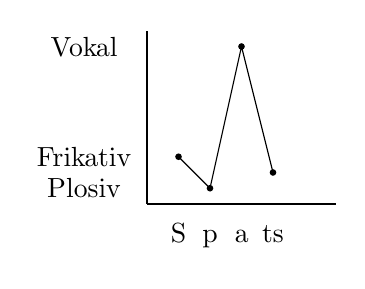
\begin{tikzpicture}[scale=0.4]
\draw[black] (-1,0) -- (5,0) ; % x axis
\draw[black] (-1,0) -- (-1,5.5); % y axis
\node at (-3,0.5) {Plosiv};
\node at (-3,1.5) {Frikativ};
\node at (-3,5) {Vokal};
\draw[black] (0,1.5) -- (1,0.5) -- (2,5) -- (3,1);
\node at (0,-1) {\strut \textipa{S}};
\node at (1,-1) {\strut \textipa{p}};
\node at (2,-1) {\strut \textipa{a}};
\node at (3,-1) {\strut \textipa{\texttoptiebar{ts}}};
\fill (0,1.5) circle [radius=3pt];
\fill (1,0.5) circle [radius=3pt];
\fill (2,5) circle [radius=3pt];
\fill (3,1) circle [radius=3pt];
\end{tikzpicture}
\pause
\hfill
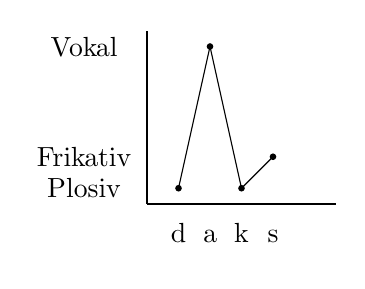
\begin{tikzpicture}[scale=0.4]
\draw[black] (-1,0) -- (5,0) ; % x axis
\draw[black] (-1,0) -- (-1,5.5); % y axis
\node at (-3,0.5) {Plosiv};
\node at (-3,1.5) {Frikativ};
\node at (-3,5) {Vokal};
\draw[black] (0,0.5) -- (1,5) -- (2,0.5) -- (3,1.5);
\node at (0,-1) {\strut \textipa{d}};
\node at (1,-1) {\strut \textipa{a}};
\node at (2,-1) {\strut \textipa{k}};
\node at (3,-1) {\strut \textipa{s}};
\fill (0,0.5) circle [radius=3pt];
\fill (1,5) circle [radius=3pt];
\fill (2,0.5) circle [radius=3pt];
\fill (3,1.5) circle [radius=3pt];
\end{tikzpicture}
\hfill\mbox{}
\vfill
\pause
\hfill
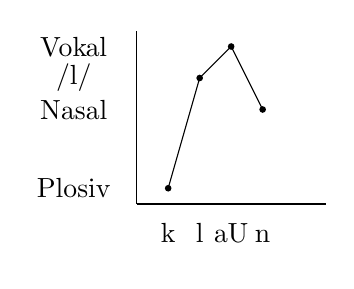
\begin{tikzpicture}[scale=0.4]
\draw[black] (-1,0) -- (5,0) ; % x axis
\draw[black] (-1,0) -- (-1,5.5); % y axis
\node at (-3,0.5) {Plosiv};
\node at (-3,3) {Nasal};
\node at (-3,4) {\textipa{/l/}};
\node at (-3,5) {Vokal};
\draw[black] (0,0.5) -- (1,4) -- (2,5) -- (3,3);
\node at (0,-1) {\strut \textipa{k}};
\node at (1,-1) {\strut \textipa{l}};
\node at (2,-1) {\strut \textipa{\texttoptiebar{aU}}};
\node at (3,-1) {\strut \textipa{n}};
\fill (0,0.5) circle [radius=3pt];
\fill (1,4) circle [radius=3pt];
\fill (2,5) circle [radius=3pt];
\fill (3,3) circle [radius=3pt];
\end{tikzpicture}
\hfill
\pause
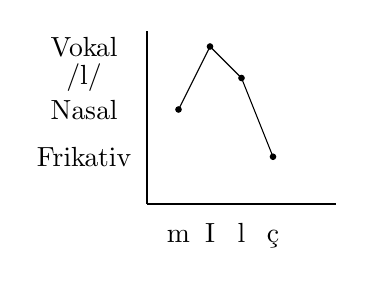
\begin{tikzpicture}[scale=0.4]
\draw[black] (-1,0) -- (5,0) ; % x axis
\draw[black] (-1,0) -- (-1,5.5); % y axis
\node at (-3,1.5) {Frikativ};
\node at (-3,3) {Nasal};
\node at (-3,4) {\textipa{/l/}};
\node at (-3,5) {Vokal};
\draw[black] (0,3) -- (1,5) -- (2,4) -- (3,1.5);
\node at (0,-1) {\strut \textipa{m}};
\node at (1,-1) {\strut \textipa{I}};
\node at (2,-1) {\strut \textipa{l}};
\node at (3,-1) {\strut \textipa{\c{c}}};
\fill (0,3) circle [radius=3pt];
\fill (1,5) circle [radius=3pt];
\fill (2,4) circle [radius=3pt];
\fill (3,1.5) circle [radius=3pt];
\end{tikzpicture}
\hfill\mbox{}
\vfill
\end{frame}


%%%%%%%%%%%%%%%%%%%%%%%%%%%%%%%%%%
\begin{frame}
\frametitle{Übung -- Lösung}

\begin{itemize}
\item Erklären Sie die Ungrammatikalität der folgenden Silben:\\
(Vokal $>$ \textipa{/\textscr /} $>$ \textipa{/l/} $>$ Nasal $>$ Frikativ $>$ Plosiv)
\begin{exe}
	\exr{ex:lbat}
	\settowidth\jamwidth{XXXXXXXXXXXXXXXXXXXXXXXXXXXXXXXXXX}
	\begin{xlist}
		\ex[*]{ \textipa{[lbat]}\loesung{2}{\textipa{[l]} vor \textipa{[b]} im Onset} }
		\ex[*]{ \textipa{[blabl]}\loesung{3}{\textipa{[b]} vor \textipa{[l]} in der Koda $+$ Auslautverhärtung} }
		\ex[*]{ \textipa{[{\textscr}mapt]}\loesung{4}{\textipa{[\textscr ]}vor \textipa{[m]} im Onset } }
		\ex[*]{ \textipa{[ki:l\textscr]}\loesung{5}{\textipa{[l]} vor \textipa{[\textscr ]} in der Koda} }
		\ex[*]{ \textipa{[ngang]}\loesung{6}{\textipa{[n]} vor \textipa{[g]} im Onset $+$ reg. velare Nasalassimiliation } \loesung{6}{$+$ g-Tilgung}}
		\ex[*]{ \textipa{[krafm]}\loesung{7}{\textipa{[f]} vor \textipa{[m]} in der Koda} }
		\ex[*]{ \textipa{[elat]}\loesung{8}{2 Silben (2 Nuklei) $+$ Knacklauteinsetzung} }
		\ex[*]{ \textipa{[plaml]}\loesung{9}{\textipa{[m]} vor \textipa{[l]} in der Koda} }
		\ex[*]{ \textipa{[nfatl]}\loesung{10}{\textipa{[n]} vor \textipa{[f]} im Onset $+$ \textipa{[t]} vor \textipa{[l]} in der Koda} }
	\end{xlist}
\end{exe}

\end{itemize}

\end{frame}



%%%%%%%%%%%%%%%%%%%%%%%%%%%%%%%%%%%
%%%%%%%%%%%%%%%%%%%%%%%%%%%%%%%%%%%
\section{Hausaufgaben}

%%%%%%%%%%%%%%%%%%%%%%%%%%%%%%%%%%
%% HA 1 - 03b Phonologie
%%%%%%%%%%%%%%%%%%%%%%%%%%%%%%%%%%

\begin{frame}
\frametitle{Hausaufgabe -- Lösung}

\begin{itemize}
	\item[1.]{Geben Sie die standarddeutsche \textbf{phonetische Transkription} für folgende Wörter an:}
	
	\begin{exe}
		\exr{ex:03bHA1}
		\begin{xlist}
		\settowidth\jamwidth{XXXXXXXXXXXXXXXXXXXXXXXXXXXXXX}
			\ex Spitzenschuhe \loesung{2}{\textipa{['SpI\textsubdot{\t{ts}}@n.Su:.@]}}
			\ex Endausscheidung \loesung{3}{\textipa{['PEnt.P\texttoptiebar{aU}s.S\texttoptiebar{aI}.dUN]}}
			\ex Platzanweiser \loesung{4}{\textipa{['pla\texttoptiebar{ts}.Pan.v\texttoptiebar{aI}.z5]}}
			\ex verzweifeln \loesung{5}{\textipa{[fE5.'\texttoptiebar{ts}v\texttoptiebar{aI}.f@ln]}}
			\ex abverlangen \loesung{6}{\textipa{['Pap.fE5.la\.N@n]}}
			\ex Überarbeitung \loesung{7}{\textipa{[Py:.b5.'Pa\;R.b\texttoptiebar{aI}.tUN]}}
			\ex Zugeständnis \loesung{8}{\textipa{['\texttoptiebar{ts}u:.g@.StEnt.nIs]}}
		\end{xlist}
	\end{exe}

\end{itemize}

\end{frame}
%%%%%%%%%%%%%%%%%%%%%%%%%%%%%%%%%

\begin{frame}{Hausaufgabe -- Lösung}

\begin{itemize}
	\item[2.]{Erläutern Sie anhand der folgenden Beispiele, unter welchen Bedingungen die \textbf{Auslautverhärtung} im Deutschen stattfindet.}

	\begin{exe}
		\exr{ex:03bHA2}
		\begin{xlist}
		\settowidth\jamwidth{XXXXXXXXXXXXXXXXXXXXXXXXXXXXXXX}
			\ex Wand -- Wände \loesung{2}{sth. Plosive am Wortende}
			\ex lesen -- lesbar \loesung{3}{generell am Silbenende}
			\ex sagen -- sagst \loesung{4}{betrifft \emph{alle} sth. Plosive in der Koda}
			\ex Roggen \loesung{5}{jedoch keine Silbengelenke}
		\end{xlist}
	\end{exe}

\end{itemize}

\end{frame}


%%%%%%%%%%%%%%%%%%%%%%%%%%%%%%%%%%
\begin{frame}{Hausaufgabe -- Lösung}

\begin{itemize}
\item[3.]{Geben Sie fünf verschiedene \textbf{phonetische oder phonologische Prozesse} an, die in dem folgenden Satz -- teilweise nur bei schnellerem Sprechen -- beobachtet werden können.} 

\begin{exe}
	\exr{ex:03bHA3}
	\begin{quote}
	Um die fünf Haken in regelmäßigen Abständen an die Wand schrauben zu können, sollten Sie sich Bohrmaschine, Wasserwaage, Zollstock und Dübel bereitgelegt haben und auf keinen Fall die Nerven verlieren, bevor Sie nicht befestigt sind.
	\end{quote}
\end{exe}


\begin{description}
	\item[\alertgreen{\textbf{Beispiele:}}] ~

\alertgreen{
	regressive Nasalassimilation in \emph{fünf}: \textipa{[fY\textbf{m}f]}\\
	progressive Nasalassimilation nach Schwa-Elision (feeding) in \emph{Haken}: \textipa{[hak\textbf{N}]}\\
	Auslautverhärtung in \emph{Wand}: \textipa{[van\textbf{t}]}\\
	progressive Nasalassimilation nach Schwa-Elision (feeding) in \emph{schrauben}: \textipa{[S\;R\t{aU}b\textbf{m}]}\\
	g-Spirantisierung in \emph{befestigt}: \textipa{[b@fEstI\textbf{\c{c}}t]}\\
	r-Vokalisierung in \emph{Bohrmaschine}: \textipa{[bo\textbf{5}maSi:n@]}
}						
		\end{description}

\end{itemize}

\end{frame}


%%%%%%%%%%%%%%%%%%%%%%%%%%%%%%%%%%%
\begin{frame}{Hausaufgabe -- Lösung}

\begin{itemize}	
\item[4.]{Illustrieren Sie den deutschen phonemischen Kontrast der folgenden Phoneme durch \textbf{Minimalpaare}, wobei der Kontrast (wenn möglich) ein Mal initial, ein Mal final vorkommen soll.

Beispiel: \textipa{[p]} -- \textipa{[f]} Paul -- faul (Initialposition), Laub -- Lauf (Finalposition)}

\begin{exe}
	\exr{ex:03bHA4}
	\settowidth\jamwidth{XXXXXXXXXXXXXXXXXXXXXXXXXXXXXXXXXXXX}
	\begin{xlist}
		\ex \textipa{[m]} -- \textipa{[n]} \loesung{2}{muss -- Nuss, beim -- Bein}
		\ex \textipa{[p]} -- \textipa{[b]} \loesung{3}{Pass -- Bass}
			\loesung{3}{(wegen Auslautverhärtung kein finaler Kontrast möglich)}
		\ex \textipa{[h]} -- \textipa{[v]} \loesung{4}{heiß -- weiß (\textipa{[h]} kommt nicht final vor)}
		\ex \textipa{[n]} -- \textipa{[N]} \loesung{5}{Sinn -- sing (\textipa{[N]} kommt nicht initial vor)}
		\ex \textipa{[f]} -- \textipa{[v]} \loesung{6}{Fass -- was}
			\loesung{6}{(wegen Auslautverhärtung kein finaler Kontrast möglich)}
	\end{xlist}
\end{exe}
		
\end{itemize}

\end{frame}

%% -*- coding:utf-8 -*-

%%%%%%%%%%%%%%%%%%%%%%%%%%%%%%%%%%%%%%%%%%%%%%%%%%%%%%%%%


\def\insertsectionhead{\refname}
\def\insertsubsectionhead{}

\huberlinjustbarfootline


\ifpdf
\else
\ifxetex
\else
\let\url=\burl
\fi
\fi
\begin{multicols}{2}
{\tiny
%\beamertemplatearticlebibitems

\bibliography{gkbib,bib-abbr,biblio}
\bibliographystyle{unified}
}
\end{multicols}





%% \section{Literatur}
%% \begin{frame}[allowframebreaks]
%% \frametitle{Literatur}
%% 	\footnotesize

%% \bibliographystyle{unified}

%% 	%German
%% %	\bibliographystyle{deChicagoMyP}

%% %	%English
%% %	\bibliographystyle{chicago} 

%% 	\bibliography{gkbib,bib-abbr,biblio}
	
%% \end{frame}


%%%%%%%%%%%%%%%%%%%%%%%%%%%%%%%%%%%
%\begin{frame}
%\textcolor{white}{
%\ea\label{ex:lbat}
%\z
%\ea\label{ex:03bHA1}
%\z
%\ea\label{ex:03bHA2}
%\z
%\ea\label{ex:03bHA3}
%\z
%\ea\label{ex:03bHA4}
%\z
%}
%\end{frame}

\end{document}